\documentclass[useAMS,usenatbib,referee]{biom}

\usepackage{amsmath}
\usepackage[figuresright]{rotating}

\graphicspath{{include/}}

\def\bSig\mathbf{\Sigma}
\newcommand{\VS}{V\&S}
\newcommand{\tr}{\mbox{tr}}

\newcommand{\blind}{1} % 0 = not blind, 1 = blind

%\newcommand{\Stan}{{\tt Stan}}
\newcommand{\Stan}{Stan}
\newcommand{\RStan}{{\tt RStan}}
\newcommand{\edgeR}{{\tt edgeR}}
\newcommand{\baySeq}{{\tt baySeq}}
\newcommand{\ShrinkBayes}{{\tt ShrinkBayes}}
\newcommand{\RNAseq}{RNA-seq}

%\renewcommand{\gamma}{c}


\title{Empirical Bayes analysis of \RNAseq{} data for detection of gene expression heterosis}

\if0\blind{
\author{Jarad Niemi$^*$\email{niemi@iastate.edu}, 
Eric Mittman, 
Will Landau, and 
Dan Nettleton \\
Department of Statistics, Iowa State University, Ames, Iowa, U.S.A.}
} \fi

\begin{document}

\date{{\it Received July} 2015} 

\pagerange{\pageref{firstpage}--\pageref{lastpage}} 
\volume{VV}
\pubyear{YYYY}
\artmonth{MM}
\doi{x}

\label{firstpage}

\begin{abstract}
Heterosis, or hybrid vigor, refers to the enhancements in the phenotype of hybrid progeny relative to their inbred parents. Although the heterosis phenomenon is extensively utilized in agriculture, the molecular basis of heterosis is still largely unknown. In an effort to understand phenotypic heterosis at the molecular level, researchers have begun to measure transcript abundance levels of thousands of genes in parental inbred lines and their hybrid offspring using RNA sequencing (\RNAseq{}) technology.  The resulting data allow researchers to search for evidence of gene expression heterosis as one potential molecular mechanism underlying heterosis of agriculturally important traits.  The null hypotheses of greatest interest in testing for gene expression heterosis are composite null hypotheses that are difficult to test with standard statistical approaches for \RNAseq{} analysis. To address these shortcomings, we develop a hierarchical negative binomial model and draw inferences using a computationally tractable empirical Bayes approach to inference. We demonstrate improvements over alternative methods via a simulation study based on a maize experiment and then analyze that maize experiment with our newly proposed methodology. 
% This article has supplementary material online.
\end{abstract}

\begin{keywords}
Hierarchical model; Negative binomial; \RNAseq{}; Bayesian LASSO; Parallel computing; \Stan{}.
\end{keywords}

\maketitle

%  A maximum of six (6) tables or figures combined is often required.''

\section{Introduction}
\label{s:intro}

Heterosis, or hybrid vigor, occurs when hybrid progeny display phenotypes that are superior to the average phenotypes of their parents.  The heterosis phenomenon was scientifically documented in plants by \cite{darwin1876effects} and has long been used to improve agricultural production. Overdominance is a particularly extreme case of heterosis where the hybrid phenotype lies outside the range of the parental phenotypes. One classic example involves hybrid maize offspring that are taller, faster to mature, and yield considerably more grain than their inbred parents \citep{hallauer1981quantitative, hallauer2010quantitative}.  Despite intensive study and successful use of heterosis in agriculture, the basic molecular genetic mechanisms remain largely unknown \citep{coors1999genetics, lippman2007heterosis}. One potential explanation, known as gene expression heterosis, is enhanced expression of one or more genes in hybrids compared to their inbred parents \citep{swanson2006all, springer2007allelic}.

Recently, \cite{ji2014estimation} introduced an approach to assess gene expression heterosis using microarray data under the assumption that these data are continuous. They built a normal hierarchical model for microarray measurements of transcript abundance that allows borrowing of information across genes to estimate means and variances. They introduced an empirical Bayes framework that first estimates model hyperparameters, then estimates the posterior distribution for gene-specific parameters conditional on those hyperparameters, and finally computes heterosis probabilities based on integrals of regions under this posterior. This development was necessary due to the composite null hypotheses in tests for heterosis. These hypotheses, which many available methods do not fully accommodate, remain a challenge in the transition from continuous measurements of transcript abundance to count-based measurements that arise from RNA sequencing (\RNAseq{}) technology. Building on the work of \citeauthor{ji2014estimation} with the normal data model, we construct a hierarchical model based on a negative binomial data model. We also utilize an empirical Bayes approach to obtain estimates of the hyperparameters and the posterior distributions for the gene-specific parameters conditional on those hyperparameters. 

The remainder of the paper proceeds as follows. Section \ref{s:method} presents the proposed hierarchical model, an empirical Bayes method of estimating the parameters, and the calculation of posterior probabilities of overdominance. Section \ref{s:simulation} presents a simulation study based on a maize experiment and compares our approach to alternative methods. Section \ref{s:maize} analyzes a maize experiment where phenotypic heterosis is well established and identifies genes demonstrating expression heterosis. The data and code necessary to perform this analysis are available in the Supplemental Material. Section \ref{s:discussion} summarizes the work and suggests directions for future research.


\section{Empirical Bayes identification of gene expression heterosis from \RNAseq{} read counts}
\label{s:method}

We consider an RNA sequencing (\RNAseq{}) experiment that involves at least three genetic varieties: two parental varieties (P1 and P2) and a cross between these two varieties called the hybrid (H). For each variety, replicate RNA samples are isolated and assessed for quality. Complementary DNA (cDNA) libraries, consisting of short cDNA fragments derived from RNA, are constructed. Then, next generation sequencing technology is used to determine the \emph{reads}, or nucleotide sequences, in the cDNA libraries. These reads are processed using bioinformatic algorithms to match the reads to genes, or specific gene transcripts, exons, microRNAs, etc. The results of read processing are summarized by a gene $\times$ sample matrix of counts. See \cite{datta2014statistical} for more details on \RNAseq{} experiments and data from a statistical perspective, and see \cite{paschold2012complementation} for the biological background behind the use of \RNAseq{} to study gene expression heterosis.

To use \RNAseq{} counts to identify genes displaying expression heterosis, we build a hierarchical model to borrow information across gene-variety means and across gene-specific overdispersion parameters, estimate the parameters using an empirical Bayes procedure implemented in the statistical software \Stan{}, and calculate empirical Bayes posterior probabilities for heterosis. 


\subsection{Hierarchical model for \RNAseq{} counts}
\label{s:model}

Let $Y_{gvi}$ be the count for gene $g=1,\ldots,G$, variety $v=1,\ldots,V$, and replicate $i=1,\ldots,n_v$.  We assume
\begin{equation} 
Y_{gvi} \stackrel{ind}{\sim} \mbox{NB}\left(e^{\mu_{gv}+\gamma_{vi}},e^{\psi_g}\right), 
\label{e:data}
\end{equation}
where NB$(\xi,e^\psi)$ indicates a negative binomial distribution with expectation $\xi$ and variance $\xi+e^\psi\xi^2$, and $ind$ indicates the observations are conditionally independent.  As shown in equation \eqref{e:data}, our data model involves gene-specific overdispersion $\psi_g$ and a mean that depends on the gene-variety combination through $\mu_{gv}$ and on the sample though  $\gamma_{vi}$.  The $\mu_{gv}$ terms are of primary scientific interest; the $\gamma_{vi}$ terms are normalization factors that account for differences in the thoroughness of sequencing from sample to sample. 

Following \cite{ji2014estimation}, we reparameterize the gene-variety mean structure into the gene-specific parental average ($\phi_g$), half-parental difference ($\alpha_g$), and hybrid difference ($\delta_g$). Specifically, for our heterosis where $V=3$, we let $v=1,2$ indicate the two parental varieties and $v=3$ indicate the hybrid, then
\[ \phi_g = \frac{\mu_{g1}+\mu_{g2}}{2}, \quad 
\alpha_g = \frac{\mu_{g1}-\mu_{g2}}{2}, \quad \mbox{and} \quad
\delta_g = \phi_g-\mu_{g3}. \]

We assume a hierarchical model for the gene-specific mean parameters and overdispersion parameters. The parental averages and overdispersion parameters are assumed to follow normal distributions, i.e.
\[ 
%\gamma_{vi} \stackrel{ind}{\sim} N(0,\sigma_\gamma^2), \quad 
\phi_g \stackrel{ind}{\sim} N(\eta_\phi, \sigma_\phi^2), \quad \mbox{and}\quad 
\psi_g \stackrel{ind}{\sim} N(\eta_\psi,\sigma_\psi^2). 
\]
To allow for more shrinkage with the half-parental and hybrid differences, we use a Laplace (or double exponential prior) and thus implement a Bayesian LASSO \citep{park2008bayesian}, i.e. 
\[ 
\alpha_g \stackrel{ind}{\sim} La(\eta_\alpha, \sigma_\alpha) \qquad \mbox{and} \qquad
\delta_g \stackrel{ind}{\sim} La(\eta_\delta, \sigma_\delta) 
\]
where $\alpha\sim La(\eta,\sigma)$ has a probability density function given by $La(\alpha;\eta,\sigma) = \exp(-|\alpha-\eta|/\sigma)/2\sigma$ with expectation $\eta$ and variance $2\sigma^2$. We assume \emph{a priori} independence amongst the parental averages, half parental differences, hybrid differences, and overdispersion parameters.

\subsection{Empirical Bayes}
\label{s:ebayes}

Initial attempts to estimate the models above via Markov chain Monte Carlo (MCMC) failed due to high computational costs and poor mixing in the resulting chains. For example, we implemented the model in the statistical software \Stan{} (discussed at the end of this section), ran the MCMC on a simulated data set with 10,000 genes for 2 months on a state-of-the-art linux server, and obtained potential scale reduction factors that suggested we would need to run at least ten times as long to obtain convergence. Although there are certainly improvements that could be made to decrease computational costs and improve mixing, we opted for an empirical Bayes approach. This approach may be a reasonable approximation to a fully Bayesian approach when estimating models with large numbers of genes as the posterior distributions for the hyperparameters may be tightly peaked. 

We categorize the parameters of the model in Section \ref{s:model} into gene-specific parameters $\theta = (\theta_1,\ldots,\theta_G)$ where $\theta_g = (\phi_g,\alpha_g,\delta_g,\psi_g)$, normalization factors $\gamma = (\gamma_{11},\ldots,\gamma_{Vn_V})$, and hyperparameters $\pi = (\eta, \sigma)$ where $\eta=(\eta_\phi,\eta_\alpha,\eta_\delta, \eta_\psi)$ and $\sigma=(\sigma_\phi,\sigma_\alpha,\sigma_\delta,\sigma_\psi)$. We obtain estimates for the hyperparameters and then base gene-specific inference on the posterior conditional on these estimates. 

To obtain normalization factors $\hat{\gamma}$, we use the weighted trimmed mean of $M$ values (TMM) method of \cite{robinson2010scaling}. We then use the methods of \cite{mccarthy2012differential}, to obtain genewise dispersion estimates, $\hat{\psi}_g$, and their generalized linear model methods to obtain estimates for the remaining gene-specific parameters, i.e. $\hat{\phi}_g$, $\hat{\alpha}_g$, and $\hat{\delta}_g$. Using $\hat{\theta}_g = (\hat{\phi}_g,\hat{\alpha}_g,\hat{\delta}_g,\hat{\psi}_g)$, we estimate hyperparameters for the location and scale parameters in the hierarchical model using a central method of moments approach, e.g. $\hat{\eta}_\phi = \sum_{g=1}^G \hat{\phi}_g/G$ and $\hat{\sigma}_\phi^2 = \sum_{g=1}^G (\hat{\phi}_g - \hat{\eta}_\phi)^2/(G-1)$ (and similarly for $\hat{\eta}_\psi$ and $\hat{\sigma}_\psi$) and $\hat{\eta}_\alpha = \sum_{g=1}^G \hat{\alpha}_g/G$ and $2\hat{\sigma}_\alpha^2 = \sum_{g=1}^G (\hat{\alpha}_g - \hat{\eta}_\alpha)^2/(G-1)$ (and similarly for $\hat{\eta}_\delta$ and $\hat{\sigma}_\delta$). 

Conditional on the estimated normalization factors $\hat{\gamma}$ and hyperparameters $\hat{\pi}$, we perform a Bayesian analysis to re-estimate the gene-specific parameters and describe their uncertainty. Conditional on $\hat{\gamma}$ and $\hat{\pi}$ the gene-specific parameters are independent, i.e.
\begin{equation}
\begin{split}
p\left(\theta\left|y,\hat{\pi},\hat{\gamma}\right.\right) 
%&= \prod_{g=1}^G p\left(\theta_g\left|y_g,\hat{\pi}\right.\right) = \prod_{g=1}^G p\left(y_g\left|\theta_g,\hat{\gamma}\right.\right) p\left(\theta_g\left|\hat{\pi}\right.\right) \nonumber \\
%&\propto \prod_{g=1}^G \left[ \prod_{v=1}^V \prod_{i=1}^{n_v} NB\left(y_{gvi}\left|e^{\mu_{gv}+\hat{\gamma}_{vi}},e^{\psi_g}\right.\right) \right] p(\theta_g|\hat{\eta},\hat{\sigma}) \\
\propto \prod_{g=1}^G & \left[ \,\prod_{v=1}^V \prod_{i=1}^{n_v} \mbox{NB}\left(y_{gvi};e^{\mu_{gv}+\hat{\gamma}_{vi}},e^{\psi_g}\right)  \right. \\
&\times 
\left. \vphantom{\prod_{v=1}^V}
N(\phi_g;\hat{\eta}_\phi, \hat{\sigma}_\phi^2)
La(\alpha_g;\hat{\eta}_\alpha, \hat{\sigma}_\alpha)
La(\delta_g;\hat{\eta}_\delta, \hat{\sigma}_\delta)
N(\psi_g;\hat{\eta}_\psi, \hat{\sigma}_\psi^2) 
\right]
\label{e:condind}
\end{split}
\end{equation}
Thus, conditional posterior inference across the genes can be obtained independently and in parallel.

To perform this Bayesian analysis, we used the statistical software \Stan{} \citep{stan-software:2014} executed through the \RStan{} interface \citep{rstan-software:2014} in R \citep{R2014}. \Stan{} implements a variant of MCMC called Hamiltonion Monte Carlo \citep{neal2011mcmc} to obtain samples from the posterior in equation \eqref{e:condind}. We ran 4 simultaneous chains with random initial starting values for 1000 burnin (and tuning) iterations followed by another 1000 iterations thinned by 4 (to reduce storage space) for inference. We monitored convergence using the potential scale reduction factor and effective sample size (ESS) for $\phi_g$, $\alpha_g$, $\delta_g$, and $\psi_g$ \citep{Gelm:Rubi:infe:1992}. If the minimum ESS was less than 1000, we reran the chains with double the iterations for both burnin and inference. We continued this restarting and doubling until we obtained minimum ESS greater than 1000 for all parameters.

\subsection{Gene expression heterosis}
\label{s:gene_heterosis}

In the maize context that motivates this work, we are particularly interested in overdominance, either low-parent heterosis (LPH) or high-parent heterosis (HPH), in gene expression. 
For a specific gene $g$, LPH occurs when average expression in the hybrid is less than the average expression of either parent, i.e. $\delta_g < -|\alpha_g|$ (equivalently $\mu_{g3} < \min\{\mu_{g1},\mu_{g2}\}$), and HPH occurs when average expression in the hybrid is greater than the average expression of either parent, i.e. $\delta_g > |\alpha_g|$. 
% and high-parent  heterosis (HPH) of gene expression occurs when $\max(\mu_{g1},\mu_{g2}) < \mu_{g3}$. For simplicity, we define \emph{heterosis} of gene expression to be the event of LPH or HPH. The most important hypotheses are
% \begin{align}
% H_{g0}:&\mu_{g1}\le \mu_{g3}\le \mu_{g2} \mbox{ or } \mu_{g1}\ge \mu_{g3}\ge \mu_{g2} \mbox{\ \ vs.\ \ } \nonumber \\
% H_{g1}:&\mu_{g3}< \min(\mu_{g1},\mu_{g2}) \mbox{ or } \max(\mu_{g1},\mu_{g2}) < \mu_{g3},
% \label{e:hypotheses}
% \end{align}
% where $H_{g0}$ indicates no heterosis for gene $g$ and $H_{g1}$ indicates  heterosis for gene $g$. 
% We evaluate these hypotheses based on empirical Bayes estimates of their posterior probabilities, e.g., 
% \begin{align}
% P\left(H_{g1}|y, \hat{\pi}_{MAP}\right) &= P\left(\left.\mu_{g3}< \min(\mu_{g1},\mu_{g2}) \mbox{ or } \max(\mu_{g1},\mu_{g2}) < \mu_{g3}\right| y, \hat{\pi}_{MAP}\right) \nonumber \\
% &\approx \frac{1}{M} \sum_{m=1}^M \mathrm{I}\left(\mu_{g3}^{(m)}< \min\left(\mu_{g1}^{(m)},\mu_{g2}^{(m)}\right) \mbox{ or } \max\left(\mu_{g1}^{(m)},\mu_{g2}^{(m)}\right) < \mu_{g3}^{(m)}\right), \label{e:probs}
% \end{align}
% where $\mu_g^{(m)} = \left(\mu_{g1}^{(m)},\mu_{g2}^{(m)},\mu_{g3}^{(m)}\right)$ is the $m^{th}$ MCMC sample from the empirical Bayes posterior, and $\mathrm{I}(A)$ is 1 if A is true and 0 otherwise. 
We evaluate these probabilities based on empirical Bayes estimates of their posterior probabilities, e.g., 
\begin{equation}
%P(LPH_g|y) \approx 
P(\mbox{LPH}_g|y,\hat{\pi},\hat{\gamma}) = 
%P\left(\left. \mu_{g3} < \min\{\mu_{g1},\mu_{g2}\}\right|y,\hat{\pi},\hat{\gamma}\right) = 
P\left(\left.\delta_g < -|\alpha_g|\right|y, \hat{\pi},\hat{\gamma}\right) = \frac{1}{M} \sum_{m=1}^M \mathrm{I}\left(\delta_g^{(m)} < -\left|\alpha_g^{(m)}\right|\right), 
\label{e:probs}
\end{equation}
where $\left(\delta_g^{(m)},\alpha_g^{(m)}\right)$ is the $m^{th}$ MCMC sample from the empirical Bayes posterior, and $\mathrm{I}(A)$ is 1 if A is true and 0 otherwise. HPH probability is defined similarly with the inequality reversed and without the negative sign. We construct a ranked list of genes according to the maximum of the gene's LPH and HPH heterosis probabilities. Geneticists can use this list to prioritize future experiments to understand the molecular genetic mechanisms for heterosis.  


\subsection{Implementation in \ShrinkBayes{}} \label{s:shrinkbayes}

In addition to the approach above, we utilized \ShrinkBayes{} to estimate heterosis probabilities with two modifications described here. \ShrinkBayes{} utilizes integrated nested Laplace approximation (INLA) \citep{rue2009approximate} in combination with empirical Bayes ideas \citep{van2014shrinkbayes}. One limitation with inferential methods based on INLA is that all distributions, except for the data distribution, must have tails as light or lighter than the normal density. Thus, we cannot implement the Laplace priors for the half-parental difference ($\alpha_g$) and the hybrid difference ($\delta_g$) and instead use normal priors in this situation. An additional limitation is that INLA provides approximations to marginal posteriors for parameters or linear combinations of parameters, but not an approximation to the full posterior. Since we are interested in non-linear quantities such as $P(\delta_g > |\alpha_g||y)$, we cannot compute these directly using \ShrinkBayes{}. Instead, for \ShrinkBayes{}, we calculate heterosis probabilities conditional on posterior means for $\hat{\delta}_g$ and $\hat{\alpha}_g$, e.g. 
\[ 
% P_{\ShrinkBayes{}}(LPH_g|y) \equiv \left\{ \begin{array}{ll}
% P(\delta_g>-\alpha_g|y) & \mbox{if } \hat{\delta}_g > -\hat{\alpha}_g \ge 0 \\
% P(\delta_g>\phantom{-}\alpha_g|y) & \mbox{if } \hat{\delta}_g > \phantom{-}\hat{\alpha}_g \ge 0 \\
% 0 & \mbox{otherwise}
% \end{array} \right.
P_{\ShrinkBayes{}}(\mbox{LPH}_g|y) \equiv P(\delta_g<-\alpha_g|y)\mathrm{I}\left(\hat{\delta}_g < -\hat{\alpha}_g \le 0\right) + P(\delta_g<\alpha_g|y) \mathrm{I}\left(\hat{\delta}_g < \hat{\alpha}_g \ge 0\right).
%P_{\ShrinkBayes{}}(HPH|y) \equiv \left\{ \begin{array}{ll}
%P(\delta_g<-\alpha_g|y) & \mbox{if } \hat{\delta}_g > -\hat{\alpha}_g \ge 0 \\
%(\delta_g<\phantom{-}\alpha_g|y) & \mbox{if } \hat{\delta}_g > \phantom{-}\hat{\alpha}_g \ge 0 \\
%0 & \mbox{otherwise}
%\end{array} \right.
\]
HPH probability is defined similarly with all inequalities reversed. As before, we construct a ranked list of genes according to the maximum of the gene's LPH and HPH heterosis probabilities.
%the heterosis probability for gene $g$ is zero if $|\hat{\delta}_g| \le |\hat{\alpha}_g|$, $P(\delta_g>\alpha_g|y)$ if $\hat{\delta}_g > -\hat{\alpha}_g \ge 0$, $P(\delta_g - \alpha_g > 0 |y)$ if $\hat{\delta}_g > \hat{\alpha}_g \ge 0$, $P(\delta_g - \alpha_g < 0 |y)$ if $\hat{\delta}_g < \hat{\alpha}_g \le 0$, and $P(\delta_g + \alpha_g < 0 |y)$ if $\hat{\delta}_g < -\hat{\alpha}_g \le 0$.  



\section{Simulation study based on a maize experiment}
\label{s:simulation}

% \subsection{Coverage for our model}
% \input{../temp/analyze-heterosis/FIGURES/coverage}

To assess the efficacy of our method to identify genes demonstrating heterosis, we used a maize data set with parental varieties B73 and Mo17 and the hybrid variety (B73 $\times$ Mo17) \citep{paschold2012complementation} to determine realistic parameter values for a simulation study. Section \ref{s:maize} describes the maize dataset in detail. We compared our method to approaches using the R packages \edgeR{}, \baySeq{} \citep{hardcastle2010bayseq, hardcastle2012baySeq}, and \ShrinkBayes{} \citep{van2014shrinkbayes}.

\subsection{Constructing simulated data}
\label{s:sim_data}

We used the methods described at the beginning of Section \ref{s:ebayes} to obtain normalization factors $\hat{\gamma}$ and gene-specific parameter estimates $\hat{\theta}_g$ for all genes using the \edgeR{} package \citep{robinson2010edgeR} from Bioconductor \citep{gentleman2004bioconductor} applied to the maize data on 27,888 genes with average count at least one and at most two zero read counts for each variety across the four replicates.  This analysis produced sample-specific normalization factors of $\hat{\gamma}=
(0.074, -0.059, -0.074, -0.014, -0.014, -0.124,  0.093,  0.063,  0.021, -0.037,  0.049,  0.021)$. The  gene-specific parameter estimates were treated as the true parameter values for the simulation study so that our simulated datasets mimicked the existing structure among the gene-variety means of the original maize data. If $\hat{\delta}_g<-|\hat{\alpha}_g|$ ($\hat{\delta}_g >|\hat{\alpha}_g|$)  the gene was considered to have LPH (HPH).

Using these parameters and normalization factors, we simulated data according to the negative binomial model in \eqref{e:data} independently for each gene. For each simulation, we analyzed a subset of 25,000 genes selected randomly from genes with simulated counts at least one on average and with at most two zeros for each variety across replications.  We repeated this simulation process 10 times for each of 4, 8, and 16 replicates per variety, reusing normalization factors when necessary.  
% From Dan "Did we consider changing the number of zeros allowed when the number of reps is higher?  I like the idea of simplifying all this by just picking an average count threshold that his high enough to avoid problems.  I think that may be what others have done in the past."

\subsection{Alternative methods}
\label{s:alternative}

Existing \RNAseq{} data analysis methods are not specifically designed to identify gene expression heterosis, but we adapted the approaches in \edgeR{} and {\tt baySeq} to provide a measure of the strength of heterosis for each gene such that large values of this measure indicate support for heterosis.

\edgeR{} can be used to test for differential expression between any two varieties based on the fit of a negative binomial log-linear model \citep{robinson2007moderated, robinson2010edgeR}. To construct a measure of heterosis, we computed the maximum likelihood estimates of the $\mu_{gv}$ parameters for all genes using \edgeR{}'s built-in Fisher scoring algorithm, and then used likelihood ratio tests to calculate two $p$-values for each gene: $p_{g1}$  for testing $H_{g01}:\mu_{g1}=\mu_{g3}$ and $p_{g2}$ for testing $H_{g02}:\mu_{g2}=\mu_{g3}$. Then, for each gene, we define a new $p$-value denoted as $p_g$ and set to $p_g=1$ if the estimate of $\mu_{g3}$ falls between the estimates of $\mu_{g1}$ and $\mu_{g2}$ and $p_g=\max\{p_{g1},p_{g2}\}/2$ otherwise.  (For all relevant significance thresholds $\omega$ near 0, it can be shown that rejecting the null hypothesis of no heterosis of expression for gene $g$ whenever $p_g\leq \omega$ results in a test that is asymptotically size $\omega$.)  We then use $1-p_g$ as a final measure positively associated with strength of evidence for gene expression heterosis. 

{\tt baySeq} allows for a wider range of hypotheses for each gene, including $H^*_{g1}: \mu_{g1}=\mu_{g2}=\mu_{g3}$, $H^*_{g 2}: \mu_{g1}=\mu_{g2}$, $H^*_{g 3}: \mu_{g1}=\mu_{g3}$, $H^*_{g 4}: \mu_{g2}=\mu_{g3}$, and $H^*_{g 5}:$ all $\mu_g$'s are distinct. In a technique similar to our application of \edgeR{}, we used the posterior probabilities of these hypotheses to construct a measure of heterosis for each gene. We set this measure to zero if the maximum likelihood estimate, calculated using \edgeR{}, of $\mu_{g3}$ is between the maximum likelihood estimates of $\mu_{g1}$ and $\mu_{g2}$. Otherwise, the measure is the sum of the posterior probabilities of $H^*_{g 2}$ and $H^*_{g 5}$, the two hypotheses that allow for overdominance.



\subsection{Results}

For the methods in Sections \ref{s:ebayes}, \ref{s:shrinkbayes}, and \ref{s:alternative}, we sorted genes according to the computed measure of the strength of evidence for heterosis. From these sorted lists, we constructed receiver-operating characteristic (ROC) curves to evaluate the ability of these methods to distinguish genes with heterosis, as defined in Section \ref{s:sim_data}, 
% From Dan, "why this citation?"
from those without heterosis \citep{landau2013dispersion}. A representative set of ROC curves is shown in Figure \ref{f:roc}. 
\begin{figure}[htbp]
\centerline{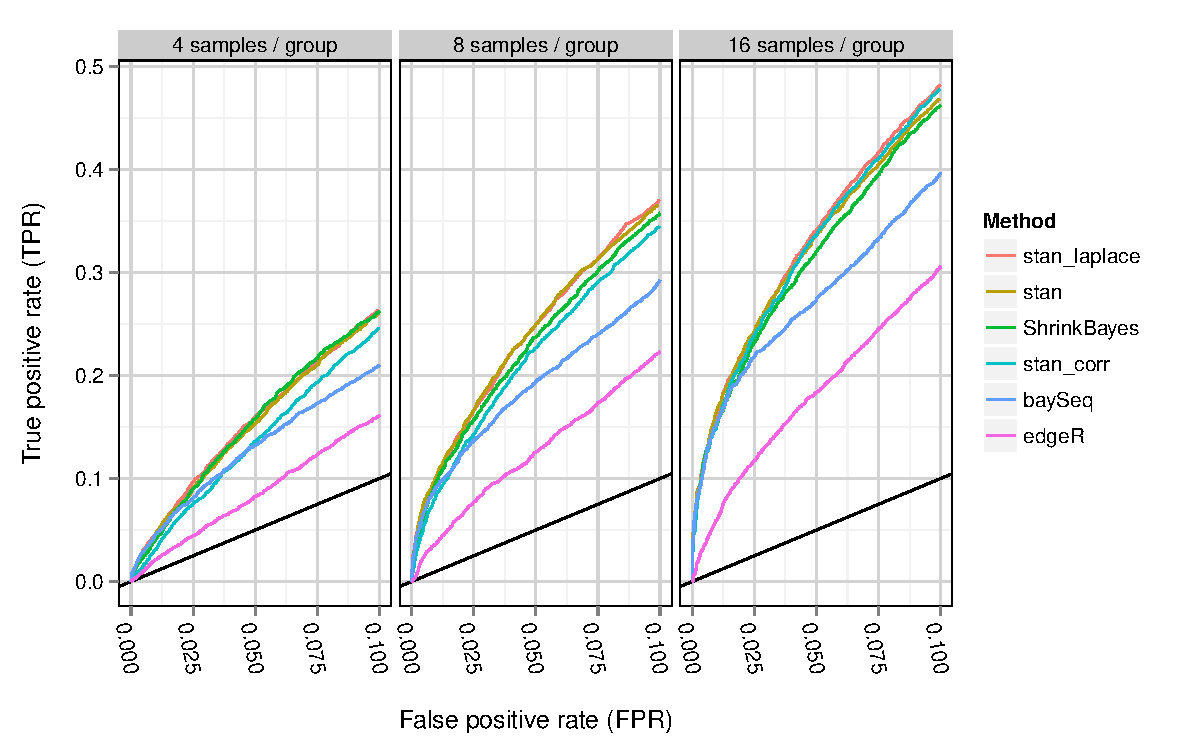
\includegraphics[width=\textwidth]{exampleROC0_1}}
\caption{Representative ROC curves for false positive rates below 0.1 for the approaches using \edgeR{} and \baySeq{} described in Section \ref{s:alternative}, the \ShrinkBayes{} approach described in Section \ref{s:shrinkbayes} and our eBayes approach described in Section \ref{s:ebayes}.}
\label{f:roc}
\end{figure}
For this simulation, we can see that the approaches based most closely on the model in Section \ref{s:model}, i.e. eBayes and \ShrinkBayes{}, provide the best true positive rate for a given false positive rate. Also, as expected, as the sample size increases, our ability to distinguish genes with heterosis from genes without improves. 


Figure \ref{f:auc} provides the area under the ROC curve below a false positive rate of 0.1 across the 10 simulations for each of the 3 different sample sizes. 
\begin{figure}
\centerline{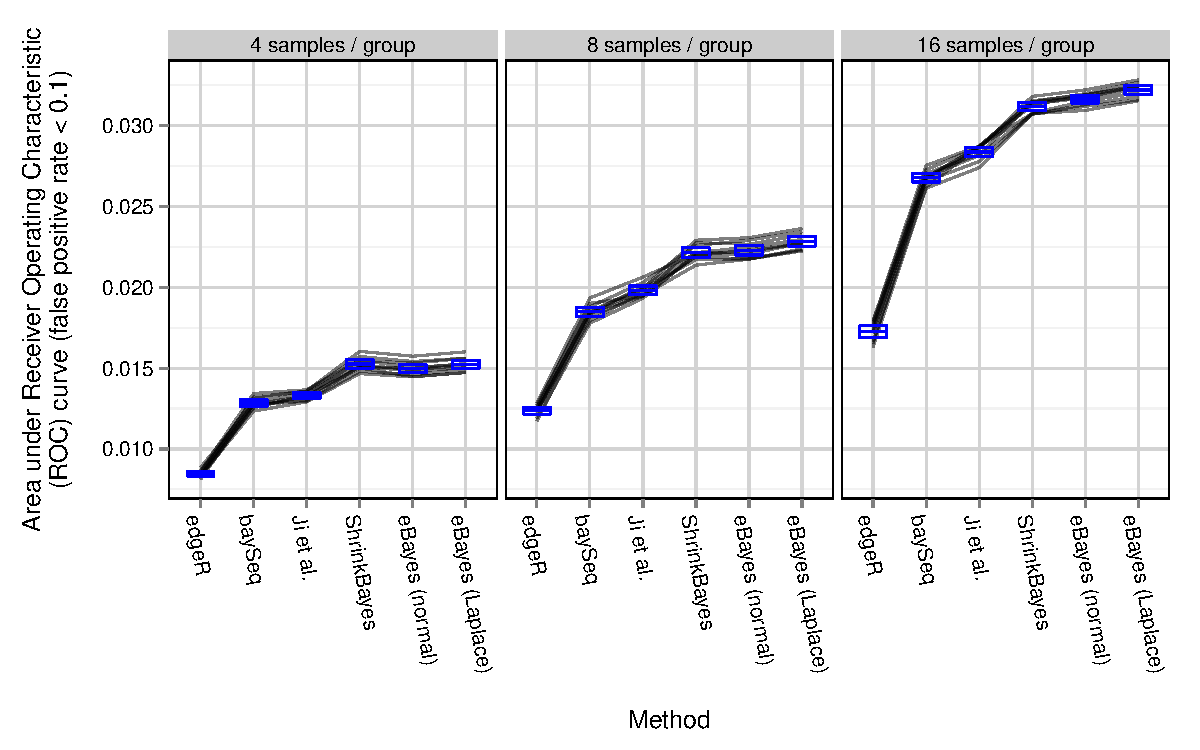
\includegraphics[width=\textwidth]{auc-facet-TRUE}}
\caption{Area under the ROC curves below a false positive rate of 0.1 for 3 different replicates per variety for the approaches using \edgeR{} and \baySeq{} described in Section \ref{s:alternative}, the \ShrinkBayes{} approach described in Section \ref{s:shrinkbayes} and our eBayes approach described in Section \ref{s:ebayes}. Each line is a different simulation while the blue box indicates mean AUC (plus or minus one standard error).}
\label{f:auc}
\end{figure}
The pattern appears to hold, with the eBayes and \ShrinkBayes{} methods outperforming the other two. With 4 replicates per variety, there does not appear to be much of a difference between \ShrinkBayes{} and our eBayes approach, but as the number of replicates increases our eBayes approach appears to improve relative to \ShrinkBayes{}.



\section{Searching for gene expression heterosis in the maize experiment}
\label{s:maize}

We used our method to analyze a maize data set \citep{paschold2012complementation} of \RNAseq{} gene expression in parental lines B73 and Mo17 and the hybrid genotype (B73$\times$Mo17). The data are available in the Supplemental Materials. Each variety had four biological replicates measured with Illumina methodology and equipment. Reads were mapped to the whole reference genome using the short reads aligner, NOVOALIGN. For more specifics, please see \cite{paschold2012complementation}. 

As explained in Section~\ref{s:sim_data}, we analyzed a set of $G=27,888$ genes for $V=3$ varieties and $n_v=4$ replicates ($v=1,2,3$). We estimated the hyperparameters to be $\hat{\eta}_\phi = 3.44$, $\hat{\sigma}_\phi = 2.74$, $\hat{\eta}_\alpha = -0.05$, $\hat{\sigma}_\alpha=0.36$, $\hat{\eta}_\delta = 0.08$, $\hat{\sigma}_\delta=0.33$, $\hat{\eta}_\psi = -2.35$, and $\hat{\sigma}_\psi=0.60$. 

Figure \ref{f:gene_specific_estimates} provides point estimates from the initial \edgeR{} estimation step and after the eBayes procedure described in Section \ref{s:ebayes}. 
\begin{figure}
\centerline{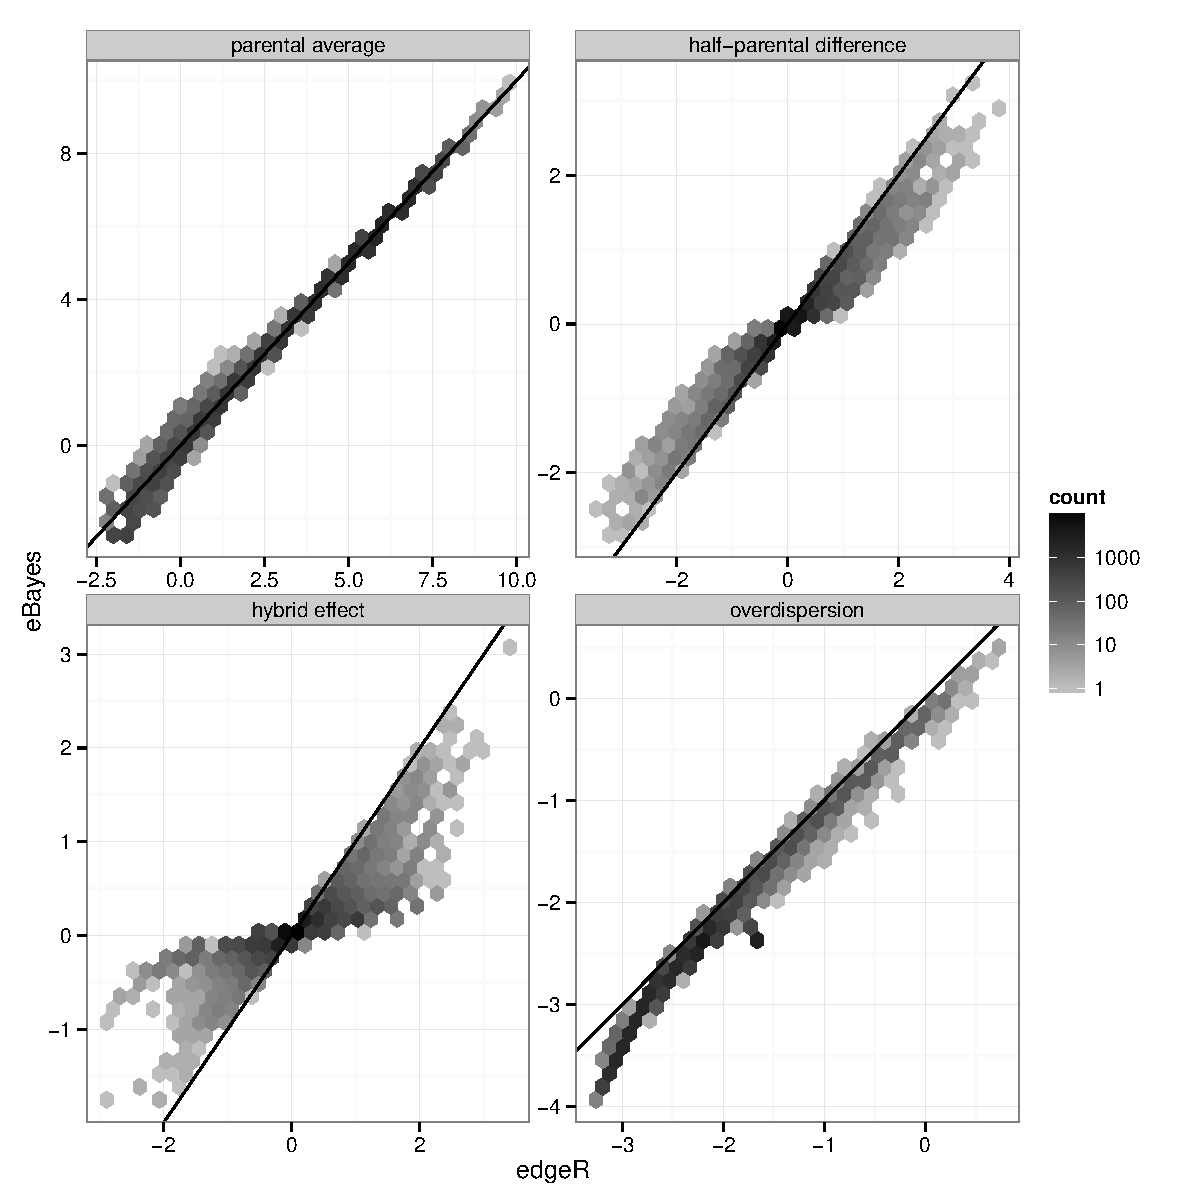
\includegraphics[width=\textwidth]{gene_specific_estimates.pdf}}
\caption{Two-dimensional histogram of point estimates from \edgeR{} and eBayes (posterior means) along with the $y=x$ diagonal.}
\label{f:gene_specific_estimates}
\end{figure}
This figure shows shrinkage for large absolute values of $\alpha$ and $\delta$ from the \edgeR{} estimation toward $\hat{\eta}_\alpha$ and $\hat{\eta}_\delta$ which are both approximately zero. The figure also shows decreased values for the overdispersion parameter with larger decreases for high and low values of overdispersion. Finally, very little, if any, shrinkage is observed for $\phi$. 

With posteriors for all parameters, we can calculate empirical Bayes posterior probabilities for LPH and HPH. For each gene, the quantity of interest is likely to be the maximum of these two probabilities. For each gene with a high probability of either HPH or LPH, the magnitude of the effect is of interest. We calculate 
\begin{equation}
% \mbox{estimated effect size}_g = \left\{ 
% \begin{array}{ll}
% \hat{\mu}_{g3} - \min(\hat{\mu}_{g1},\hat{\mu}_{g2}) & \mbox{if } \hat{\mu}_{g3} < \min(\hat{\mu}_{g1},\hat{\mu}_{g2}) \\
% \hat{\mu}_{g3} - \max(\hat{\mu}_{g1},\hat{\mu}_{g2}) & \mbox{if } \hat{\mu}_{g3} > \max(\hat{\mu}_{g1},\hat{\mu}_{g2}) \\
% 0 & \mbox{otherwise},
% \end{array} 
% \right. 
\mbox{estimated effect size}_g \equiv \left\{ 
\begin{array}{ll}
\hat{\delta}_g - |\hat{\alpha}_g| & \mbox{if } \hat{\delta}_g > \phantom{-}|\alpha_g| \\
\hat{\delta}_g + |\hat{\alpha}_g| & \mbox{if } \hat{\delta}_g < -|\alpha_g| \\
0 & \mbox{otherwise},
\end{array}.
\right. 
\label{e:effect_size}
\end{equation}
Thus, the estimated effect size is the difference between hybrid mean and the nearest parent with negative values indicating LPH and positive values indicating HPH. If the hybrid mean is estimated to be between the parents, this effect is defined to be zero. 


Figure \ref{f:volcano} provides a volcano plot, in this case a bivariate histogram, to visualize the maximum of the probabilities of LPH and HPH versus estimated effect size. 
\begin{figure}
\centerline{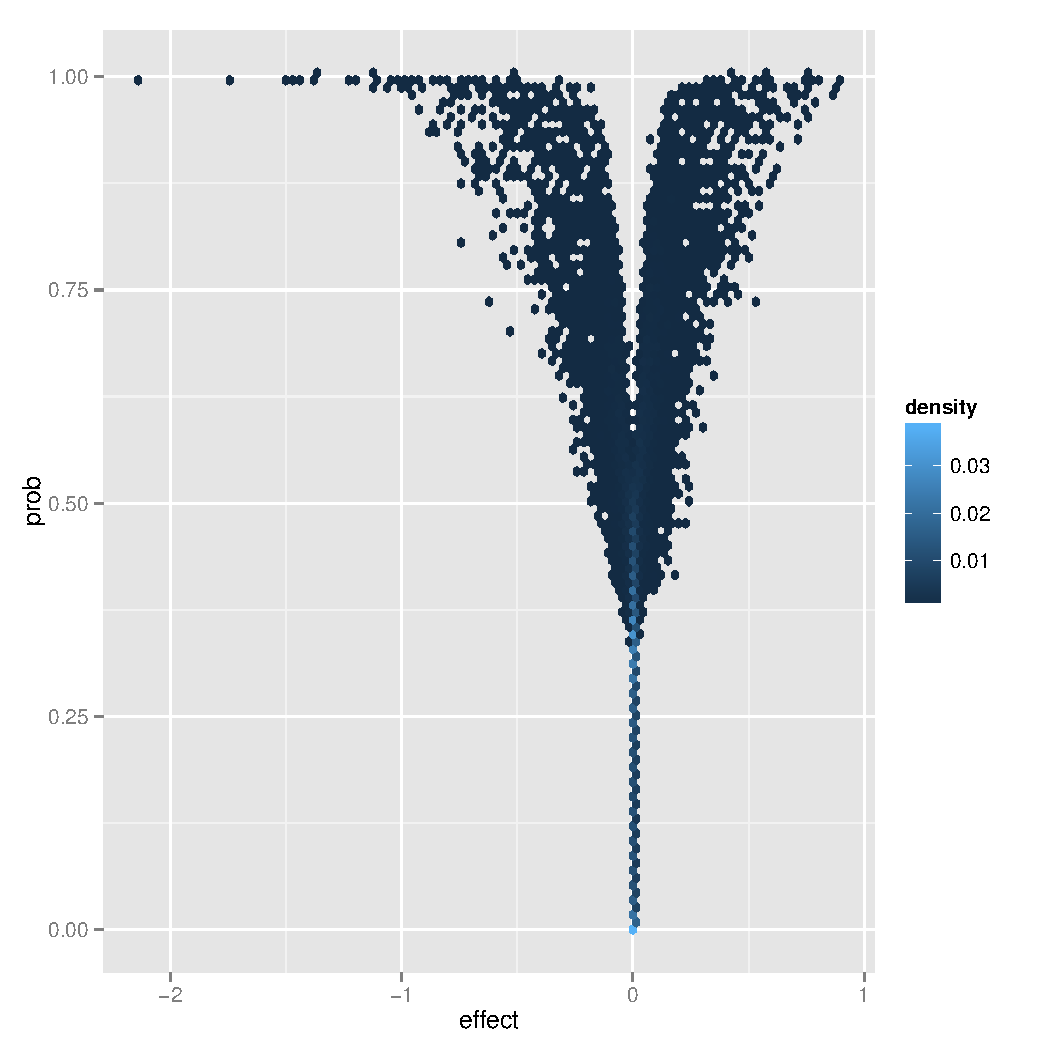
\includegraphics[width=\textwidth]{volcano}}
\caption{A bivariate histogram of the maximum of the LPH and HPH probabilities versus estimated effect size defined in equation \eqref{e:effect_size} for the B73 $\times$ Mo17 maize experiment.}
\label{f:volcano}
\end{figure}
The figure shows a ridge at an effect size of zero for probabilities below 0.5. Above a probability of 0.5, we see a prototypical volcano pattern, with increased heterosis probability corresponding to larger estimated effect sizes and no estimated effect sizes near zero for genes with high heterosis probability. We also see asymmetry, with larger negative effect sizes than positive effect sizes due to genes with hybrid counts near zero and relatively high parental counts. Genes with high estimated posterior probabilities of heterosis and large estimated effect sizes are candidates for further investigation.






\section{Discussion}
\label{s:discussion}

Geneticists speculate that gene expression heterosis is one possible explanation of phenotypic heterosis of traits, such as plant height or grain yield. Existing methods for identifying differential gene expression based on \RNAseq{} data are not directly applicable for detecting heterosis genes. \cite{ji2014estimation} introduced an empirical Bayes approach based on a hierarchical model for microarray data. We followed their approach, modified to allow for \RNAseq{} read counts as measures of transcript abundance. We developed an empirical Bayes approach based on obtaining estimates for hyperparameters followed by MCMC to estimate gene-specific parameters. The empirical Bayes posteriors can be used to estimate posterior probabilities of high and low parent heterosis. Through a simulation study, we demonstrated that this method outperformed alternative methods (that are not designed to detect heterosis), and performed comparably well with a similar model in \ShrinkBayes{}, which estimates the full posterior via INLA. We then demonstrated the use of the methodology on a maize experiment in which phenotypic heterosis is well known. 

Although our method appears to improve upon existing methods, we believe our approach can be improved by refining the hierarchical model for the gene-specific parameter distribution. Figure \ref{f:scatterplot} shows marginal and bivariate histograms for the empirical Bayes posterior means for the gene-specific parameters. 
\begin{figure}
\centerline{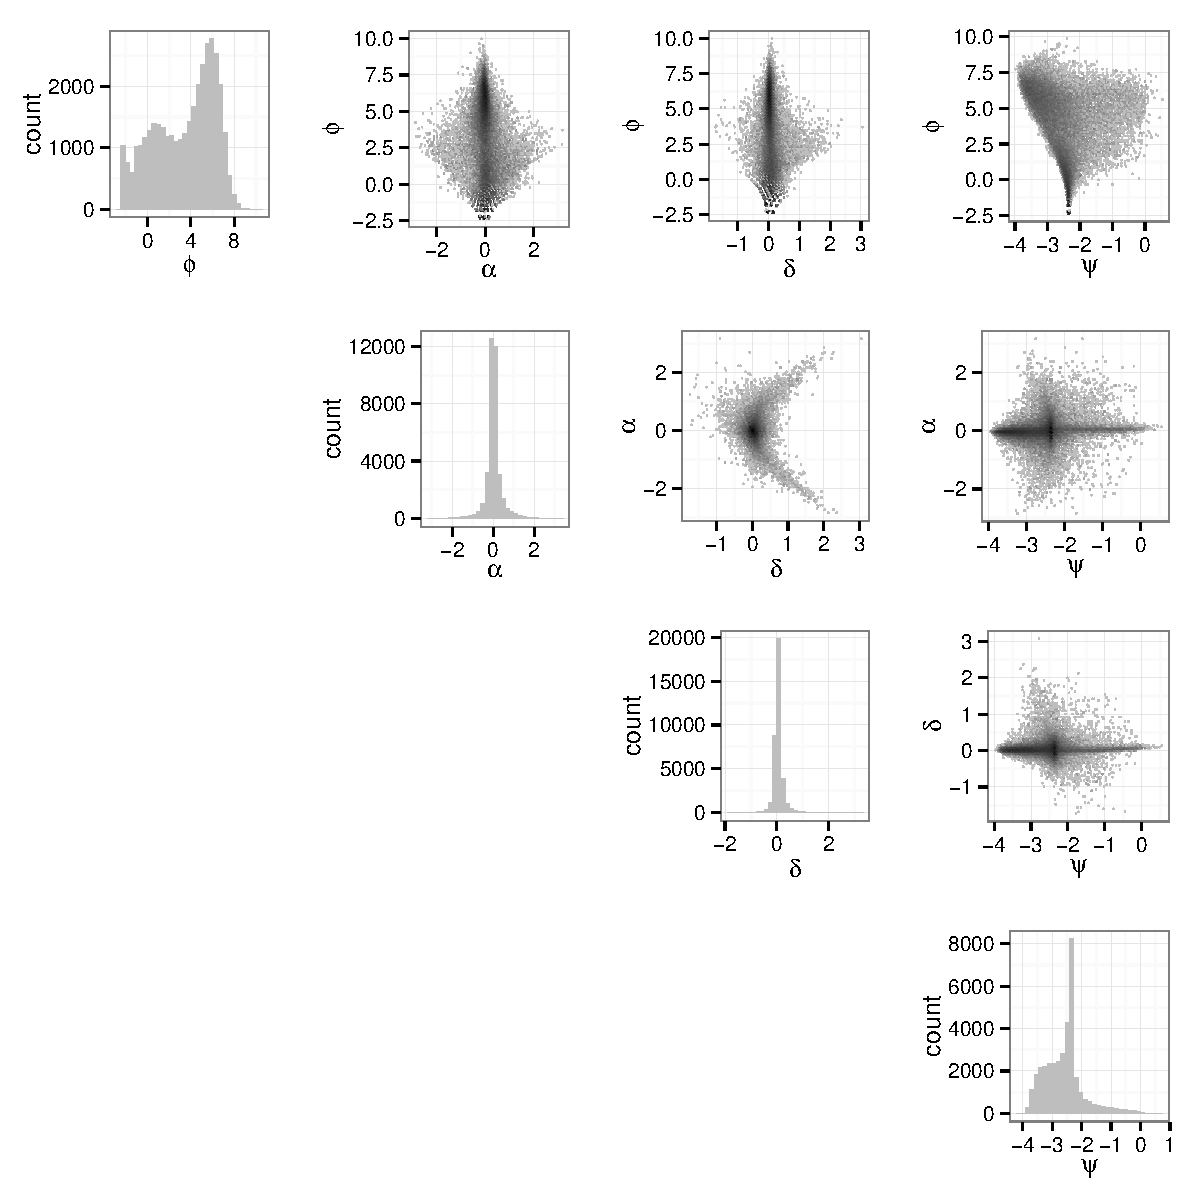
\includegraphics[width=\textwidth]{estimates}}
\caption{Marginal and bivariate histograms for gene-specific parameter posterior meansfor the B73 $\times$ Mo17 maize experiment. For reference, the marginal histograms have a dashed line indicating the appropriate marginal probability density functions in the hierarchical model with the MAP estimates.}
\label{f:scatterplot}
\end{figure}
These figures show markedly departures from marginal model assumptions, e.g. normality assumptions for $\phi_g$ and $\psi_g$, and independence assumptions, e.g. $\phi_g$ versus $\psi_g$ and $\alpha_g$ versus $\delta_g$. The plot of $\phi_g$ versus $\psi_g$ shows a pattern where the mean overdispersion decreases as the mean expression level increases. The plot of $\alpha_g$ versus $\delta_g$ shows a rotated V pattern where $\delta_g$ appears to be equal to $|\alpha_g|$. This pattern is consistent with Mendel's Law of Dominance where the hybrid has mean expression equal to the parent with higher mean expression. 

In addition to improving the hierarchical distribution, we believe better estimates of the parameters of this distribution, i.e. the hyperparameters, will also improve detection of gene-expression heterosis. Our current method, based on moment matching of essentially independently estimated gene-specific parameters provides consistent estimators as the number of replicates per variety increases. But typically the number of replicates per variety is quite small, in our data there are only four replicates per variety, and therefore asymptotic justifications are deficient. There are a variety of hyperparameter estimation approaches to explore, e.g. expectation-maximization algorithms or fully Bayesian approaches.

Notwithstanding these improvements, we believe our approach is a computationally efficient method that can immediately aid scientists who are interested in identifying candidate genes for a genetic mechanism of heterosis. 





\backmatter %  Please keep this command in your document in this position 

\if0\blind{
\section*{Acknowledgements}

The authors thank Andrew Lithio for help in implementing our model in \ShrinkBayes{}. Research reported in this publication was supported by National Institute of General Medical Sciences of the National Institutes of Health under award number R01GM109458. The content is solely the responsibility of the authors and does not necessarily represent the official views of the National Institutes of Health.
} \fi

%  If your paper refers to supplementary web material, then you MUST
%  include this section!!  See Instructions for Authors at the journal
%  website http://www.biometrics.tibs.org

%\section*{Supplementary Materials}
%The supplementary materials include three plain text files: the maize experiment data ({\tt data.csv}), a script to run our method ({\tt script.R}) on this data, and the \Stan{} model ({\tt model.stan}).  

\bibliography{jarad}
\bibliographystyle{biom}

% \appendix
% %  To get the journal style of heading for an appendix, mimic the following.
% \section{}
% \subsection{Material here}

\label{lastpage}

\end{document}
